\cotefile{69}
\scanpage{19}\mspage{15}
% @ top, lines 1–5 | text | structurel ; donnée de Q
\unsure{structurel|structural} : $\Psi$. Donc la donnée de \inserted{$Q_u$,} $Q$ avec cette \unsure{particularisation|restriction} équivaut à celle de $Q_u,P$. Pour reconstituer le graphe $C$, il faut reconstituer la notion de ``sommets liés'' sur $\{u\}\cup\underbrace{\left(\coprod_i P\wedge_{\Psi}(\mathbb F_2,p_i)\right)}_{E_{p}^*\ \deleted{\unsure{=Q_u}}}\amalg P$. On déclare :

% @ upper third, a | text | u est lié
a) $u$ est lié aux pts de $E_p^*$, et non à ceux de $P$

% @ upper third, b | text | un pt a de E
b) un \deleted{\unsure{est|un}} pt \inserted{$a$} de $E_p^*$ est lié à $\sigma a$ [i.e. si $a\in P\wedge_{\Psi}(\mathbb F_2,p_i)$, il est lié à l'autre pt $a'$ de cet ens] et à aucun autre pt de $E_p^*$

% @ upper middle, c | text | un pt a de E
c) un pt $a$ de $E_p^*$ est lié à un pt \deleted{\unsure{$a$}} $x$ de $P$ \unsure{ssi}, posant $a\in P\wedge_{\Psi}(\mathbb F_2,p_i)$, $a$ est dans l'image de $x$ par l'application canonique $P\longrightarrow P\wedge_{\Psi}(\mathbb F_2,p_i)$.

% @ middle, d | text | Deux pts x, y
d) Deux pts $x,y$ de $P$ sont liés sss l'élément $y-x=\alpha\in\Psi(Q_u)=\operatorname{Ker}(\mathbb F_{2}^{Q_u}\longrightarrow\mathbb F_2)$ est \deleted{\unsure{la}} de la forme \deleted{\unsure{$e_i$}} $e'_i$ $(i\in Q_u)$, où $e'_i=\sum_{j\in Q_u-\{i\}}e_j\in\Psi$ ($(e_j)_{j\in Q_u}$ étant la base canonique de $\mathbb F_2^{Q_u}$). Ceci ne fait que traduire le

% @ lower middle, lemma | text | Lemme Soient u ∈ C
\uline{Lemme} Soient $u\in C$, $x,y\in C-E(u)-\{u\}$. Pour que $x$ et $y$ soient liés, il \unsure{faut|f.} et s. qu'il \deleted{\unsure{l'ens|s'ensuive|puisse}} \deleted{\unsure{partie de l'ens}} \deleted{des 5 triangles $t$} \inserted{existe} \deleted{\uline{un triangle}} \inserted{(un et)} \uline{un seul} triangle de sommet $u$ tel que $t-E(x)=t-E(y)$ (NB les deux mbs sont \deleted{réduits} \inserted{de tte façon} à \uline{un} él. $\ne u$) soit \deleted{\unsure{réduis|réduits}} de cardinal 1) \unsure{SPS|SPS.|OPS} $x\ne y$.

% @ bottom, proof | text | Dém S'il n'existait
\uline{Dém} S'il n'existait aucun tel triangle, on aurait $x-y=\sum_{i\in\unsure{P_u|Q_u}}e_i$, or $\sum e_i\notin\Psi$, \inserted{car $5\ne0$ dans $\mathbb F_2$} absurde. Soit $\{u,v,w\}$ un tel triangle, \deleted{donc} $x,y$ sont liés tous deux à $v$ ou $w$ -- disons $v$. Si $y$ et $x$ sont liés, donc (avec les notations habituelles) $y=\sigma x$, on sait que pour tt $a\in E(u)^*\inserted{=E(u)-\{v,w\}}$, si $x$ lié à $a$, $\sigma x$ non lié à $a$ et inversement.
% archive sheet number: 18
\scanpage{20}\mspage{16}
% @ top, lines 1–4 | text | donc t = {u,v,w}
donc $t=\{u,v,w\}$ est unique de son espèce. Si $x$ et $y$ sont non liés, on sait qu'il existe un \inserted{(et $=$ deux)} $a\in E(u)^*$ tel que $a$ lié à la fois à $x$ et $y$, donc $t$ non unique de son espèce, cqfd.

% @ upper middle, corollary | text | Corollaire Le groupe
\uline{Corollaire} Le groupe \deleted{\unsure{des}} $W_u$ \inserted{$\subset W$} des autom de $C$ qui fixent $\unsure{a|u}$ est \deleted{\unsure{un}} isom au groupe des couples $(\unsure{\varphi|\rho},\psi)$ d'un autom $\varphi\in\unsure{\mathfrak S|\mathscr S}_{Q_u}$ de \unsure{$P_u$|$Q_u$}, et d'un $\overline{\varphi}$ autom. du \deleted{\unsure{$P$}} $\Psi_{Q_u}$ torseur $P$, où $\overline{\varphi}$ est l'autom de $\Psi_{Q_u}$ induit par $\varphi$. Donc on a une suite exacte (splittée)

% @ centre, exact sequence and vertical identifications | diagram | 1, (Ψ), W, S, 1 ; F₂⁴ and S₅
\diagram{\begin{tikzcd}[ampersand replacement=\&,column sep=large,row sep=small]
1\arrow[r,dash] \& (\Psi_{Q_u})^{\deleted{\unsure{\text{torseur}}}}\arrow[r] \& W_u\arrow[r,dash] \& \mathfrak S_{Q_u}\arrow[r,dash] \&1\\
\&\mathbb F_2^4\arrow[u,phantom,"\simeq"{description,rotate=90}] \& \&\mathfrak S_5\arrow[u,phantom,"\simeq"{description,rotate=90}] \&
\end{tikzcd}}

% @ just below fold | text | donc Wᵤ ≃ groupe de Weyl
donc $W_u\simeq$ groupe de Weyl $W_{D_5}$ de $D_5$ $(\simeq\unsure{\mathrm{so}(10)|\mathrm{SO}(10)})$ qui apparait donc comme ss-groupe d'indice 27 dans $W$ $(\simeq W_{E_6})$.

% @ lower third, NB | text | Il faudrait expliciter
\uline{NB} Il faudrait expliciter comment la donnée de $(C,u)$ permet de définir un syst. de racines $D_5$ (plongé dans le syst. de racines $E_6$ associé à $C$) -- donc définir un ens de \inserted{40} ``bases'' (=``racines'') de $C$, stable par passage à bases opposées. Or on trouve qu'il y a $40=(10.8):2$ \inserted{$=\binom{10}{2}-5$} \deleted{couples} \inserted{paires} d'éléments de $E(u)$ non liés. Or on a le

% @ foot, lemma | text | Lemme Pour tte paire
\uline{Lemme} Pour tte paire \inserted{$\{\unsure{\zeta_1|\xi_1},\unsure{\zeta_2|\xi_2}\}$} d'éléments non liés de
% archive sheet number: 19
\scanpage{21}\mspage{17}
% @ top, end of lemma | text | E(u), ∃! base
$E(u)$, $\exists!$ base $b\subset C$ telle que $b\cap E(u)=\{\unsure{\zeta|\xi}_1,\zeta_2\}$ et (si $b'$ est la base opposée) on a $b'\cap E(u)=\{\sigma\zeta_1,\sigma\zeta_{\unsure{1|2}}\}$, \deleted{\unsure{donc}} où $\sigma$ est l'autom can. d'ordre 2 de $E(u)$.

% @ above proof, NB | text | NB On aura alors
$\uparrow$ \uline{NB} On aura alors $\sigma\zeta_1=\zeta'_2$, $\sigma\zeta_2=\zeta'_1$. Alors $b\cap E(u)=\{\zeta_1,\zeta_2\}$, $b'\cap E(u)=\{\sigma\zeta_1,\sigma\zeta_2\}$.

% @ upper third, demonstration | text | Dém Soit une base
\uline{Dém} Soit une base $\{\zeta_1,\zeta_2,-\zeta_6\}$ satisfaisant à \unsure{l'énoncé}.
\margin{\unsure{principe|rappeler} plus simple plus bas}% slanted
On aura alors \deleted{\unsure{tel que}} $u$ est lié à $\zeta_1,\zeta_2,\zeta'_1,\zeta'_{\unsure{2}}$, donc $u=\zeta_{12}$, et $b\cap E(u)=\{\zeta_1,\zeta_2\}$, $b'\cap E(u)=\{\zeta'_1,\zeta'_2\}$. Pour l'existence \inserted{d'une base $b$ satisfaisant les conditions envisagées}, on note que (comme le groupe $W_u$ est transitif sur l'ens des \deleted{couples} \inserted{paires} $\{\zeta_1,\zeta_2\}$ non liées de $E(u)$ et $W=W_{E_6}$ transitif sur l'ens des $u\in C$) on peut supposer, p.r. à une base $(\bar\zeta_1,-\bar\zeta_6)$ déjà donnée, que $u=\bar\zeta_{12}$, $\zeta_1=\bar\zeta_1$, $\zeta_2=\bar\zeta_2$.

% @ centre and crossed region | text | Pour l'unicité, on note que
Pour l'unicité, on note que \deleted{\unsure{alors que} \unsure{les} $\bar\zeta'_i$ \unsure{sont} $(3\le i\le6)$ \unsure{si} $\bar\zeta_{\unsure{3}}$ est \unsure{un autre él.|un autre}  lié à $\zeta_2$ et $\unsure{\sigma\zeta_1|\zeta_1|\sigma\xi_1}=\zeta'_2$ et $\sigma\zeta_2=\zeta'_1$, et un él. de $C$ non lié à $\zeta_1,\zeta_2$ distinct de $\zeta_1$, donc est \unsure{dans|au} $\complement E(u)$, et de \unsure{même pour les} d'après ce qu'on a vu, on doit avoir que les $\bar\zeta_i,\bar\zeta'_i$ $(3\le i\le6)$ sont $\in\complement E(u)$, donc qu'ils \inserted{ceux qui} ne sont pas des $\zeta_j,\zeta'_j$,} alors que $\bar\zeta_3$ doit être non lié à $\zeta_1,\zeta_2$ et lié à $\zeta'_1,\zeta'_2$ donc ce n'est pas un $\zeta'$, ni un $\zeta_{ij}$ (car ce serait un $\zeta_{1j}$ ou $\zeta_{2j}$ pour être lié à $\zeta'_1,\zeta'_2$, mais il le serait aussi à $\zeta_1,\zeta_2$, absurde), de $=$ pour les $\bar\zeta_i$ $(3\le i\le6)$. cqfd.

% @ left of cancelled lines | diagram | two triangles sharing lower vertex, ζ₁, σζ₁, ζ₂, σζ₂
\diagram{\begin{tikzcd}[ampersand replacement=\&,execute at end picture={
\draw (0,0)--(.28,1.2) node[above left] {$\zeta_1$} --(.70,1.14) node[above right] {$\sigma\zeta_1$} --cycle;
\draw (0,0)--(1.43,.92) node[above] {$\zeta_2$} --(1.65,.54) node[right] {$\sigma\zeta_2$} --cycle;
}]\vphantom{A}\end{tikzcd}}

% @ foot, NB | text | Positions relatives
\uline{NB} Positions relatives \inserted{(à conjugaison près)} d'un $u\in C$ et d'une base $b\subset C$.

% @ foot, first case | text | (i) u ∈ b
(i) $u\in b$ \quad Pour $u\inserted{=\zeta_1}$ fixé, il y a \unsure{18|16} telles bases, corresp. \unsure{aux} au choix d'un $\zeta'_1\in C-E(u)$
\margin{$\left.\begin{aligned}r_b\unsure{(u)|{}\cdot u}&=1\\E(u)\cap b&=\varnothing\\\operatorname{card} E(u)\cap b'&=5\end{aligned}\right\}$}

% @ foot, second case | text | (ii) u ∈ b′
\deleted{\unsure{(ii)}} (ii) $u\in b'$ (base opposée) Pour $u\inserted{=\zeta'_1}$ fixé, 16 telles bases, correspondant au choix d'un $\zeta_1\in C-E(u)$
\margin{$\left.\begin{aligned}r_b\cdot u&=-1\\\operatorname{card} E(u)\cap b^{\unsure{+|*|{}}}&=5\\E(u)\cap b'&=\varnothing\end{aligned}\right\}$}

% @ foot, third case | text | (iii) u ∉ b ∪ b′
(iii) $u\notin b\cup b'$ \quad Pour $u$ fixé, il y a 40 telles bases ($r_b$ \uline{orthogonal} à $u$)
\margin{$\left.\begin{aligned}r_b\cdot u&=0\\\operatorname{card} E(u)\cap b&=2\\\operatorname{card} E(u)\cap b'&=2\end{aligned}\right\}$}

% @ foot right, total | display | 16+16+40
\[
\overline{\overline{16+16+40}}=72
\]
% archive sheet number: 20
\scanpage{22}\mspage{18 bis}
% @ top, opening | text | Soit r un entier
Soit $r$ un entier,

% @ top, a | text | Q un ens.
a) $Q$ un ens. de cardinal $r$

% @ top, b | text | Q tilde, π, Q
b) $\widetilde Q\xrightarrow{\pi} Q$ un rev. d'ordre 2 de $Q$, $\Longleftrightarrow$ un torseur \deleted{$Q$} \inserted{$\Pi$} sous $\mathbb F_2^Q$

% @ upper third, crossed c and its continuation | text | restriction du groupe structural
\deleted{c) restriction du groupe structural à $\Psi_Q=\operatorname{Ker}\bigl(\mathbb F_2^Q\longrightarrow\mathbb F_2\bigr)$, $(x_i)\longmapsto\sum x_i$,

La donnée de b), c) moyennant a), revient à la donnée d'un torseur $P$ sous $\Psi_Q$.

On va associer à ceci un ens de racines de type $D_r$.}

% @ upper middle, new a | text | produit scalaire
a) Soit $(x,y)$ le produit scalaire sur $\mathbb Z^Q$ défini pour $x,y\in Q$ par
% @ upper middle, cases | display | x.y = 0, 1, −1
\[
x.y=\begin{cases}0&\text{si }\deleted{\unsure{y}}\quad y\ne x,\sigma x\ \text{i.e. }\pi(x)\ne\pi(y)\\
1&\text{si }\quad y=\sigma x\\
-1&\text{si }\quad y=x\end{cases}
\]
% @ centre, quotient | text | Soit E(Π)
Soit $E(\unsure{\Pi|P|\deleted{\Pi}})=\mathbb Z^Q/\{x\in\mathbb Z^Q\mid x.y=0\quad\forall y\in\mathbb Z^Q\}$

% @ centre, cancelled choices | text | Choisissons ; Ordonnons Q
\deleted{Choisissons un élément} \deleted{Ordonnons $Q\simeq[1,r]$ et choisissons un élément $\tilde q_{\unsure{i}}\in\widetilde Q$ sur tt $q\in Q$, \deleted{alors on aura} soit $\sigma\tilde q$ lié à $\tilde q$, $E$ $\tilde q_i^2=-1\quad\tilde q_i\tilde q_j=0$} je dis que dans $E$, $\tilde q+\sigma\tilde q=0$ \deleted{indépendant de $q$, car} car le produit scalaire \deleted{$(\sigma\tilde q+\tilde q,\tilde q')=\bigl\{$} avec $\tilde q$ est $\deleted{\unsure{+}}\unsure{-|{}}1+1$, avec $\sigma\tilde q$ est $+1-1$, et avec \deleted{\unsure{a}} $\tilde q'\ne\tilde q,\sigma\tilde q$ est $0+0$. Donc $E$ est le $\mathbb Z$-module libre de rang $r$ engendré par les $\tilde q\in\widetilde Q$, avec $\sigma\tilde q=-\tilde q$, $(\tilde q,\tilde q)=-1$, $(\tilde q,\tilde q')=0$ si $\tilde q'\ne\tilde q,\sigma\tilde q$ \ldots.

% @ lower third, roots | text | Les racines sont les différences
Les racines sont les différences mutuelles des $\tilde q-\tilde q'$, avec $\tilde q'\ne\tilde q,\sigma\tilde q=-\tilde q$

% @ foot, cubic complex | text | Supposons que Q
Supposons que $Q=\unsure{F(u)|E(u)}$, $u$ sommet d'un complexe cubique \inserted{$C$}, OPS $C$ muni d'une base $(\unsure{\zeta|\xi}_i)_{1\le i\le6}$ et \deleted{\unsure{un}} $u=\zeta'_6$, donc
% @ foot, array E(u) | display | ζ₁ through ζ₅₆
\[
E(u)=\begin{pmatrix}\zeta_1&\zeta_2&\zeta_3&\zeta_4&\zeta_5\\\zeta_{16}&\zeta_{26}&\zeta_{36}&\zeta_{46}&\zeta_{56}\end{pmatrix},
\]
% @ very bottom, generators | text | Soit E
\deleted{\unsure{c'est}} Soit $\unsure{E'|E_f}\subset\frac12 E(C)$ engendré par les \deleted{$\varepsilon_i=\frac12(\eta-2\zeta_i-\zeta_6)=\frac12(\eta-$} $\varepsilon_i=\underbrace{\frac12(\zeta_6-\eta)}_{\theta_0}+\zeta_i$, alors les diff. mutuelles dans $\widehat E(C)$ des couples d'élts non liés de $E(u)$ sont les
% archive sheet number: 21
\scanpage{23}\mspage{18 ter}
% @ top, continuation | text | ± εᵢ ± εⱼ
$\pm\varepsilon_i\pm\varepsilon_j$ $(1\le i<j\le5)$, et l'on a un isom canonique $E(\Pi)\simeq E$. De façon intrinsèque :

% @ upper third, a | text | les x + σx
a) les $x+\sigma x$ $(x\in E(u))$ sont tous égaux, soit $\theta\in\widehat E(C)$ [savoir $\theta=\eta-\unsure{\zeta|\xi|\xi'}_6$]

% @ upper third through fold, b | text | L'hom x ↦ x − ½θ
b) L'hom $x\longmapsto x-\frac12\theta$ de $E(u)$ dans $\frac12\widehat E(C)$ \unsure{induit|\deleted{induit}} un iso de $\mathbb Z^{E(u)}/N\simeq E(\Pi)$ \deleted{sur} \uline{dans} $\unsure{\deleted{\widehat{\vphantom E}}E(C)|\widehat E(C)}$, et les différences \deleted{successives} \inserted{mutuelles} \inserted{de $E(\Pi)$} d'éléments non liés de $E(u)$ sont \unsure{transformées|transformés} en les diff. mutuelles de ces éléments dans $\widehat E(C)$, lesquelles forment donc un syst. de \inserted{(40)} racines de type $D_5$ -- qui sont aussi les \inserted{40} racines de $E_6(C)$ \deleted{\unsure{ou}} $=E(C)$ \uline{orthogonales} à $u$.
% archive sheet number: 22
\scanpage{24}\mspage{18}
% @ top, check to make | text | À vérifier Les racines
\uline{À vérifier} Les racines $r_b$ orthogonales à un $u\in C$ (au nb de 40) forment un syst. de racines de type $D_5$

% @ upper third, NB | text | La donnée de (C,u,b)
\uline{NB} La donnée de $(C,u,b)$ avec $\unsure{u|b}\in C$, $b$ base ``orthogonale'' à $u$, équivaut à la donnée d'un ens $I$ de cardinal 6 (savoir $b$) et d'une partie \inserted{de $I$} $I_2$ de cardinal 2, i.e. \deleted{\unsure{de}} d'un ens \inserted{$I_2$} de cardinal 2 et d'un autre $I_4$ de cardinal 4. \deleted{Pour un système $(C,u,\{b,b'\})$, il faut se donner} \inserted{Groupe d'autom $\unsure{\mathfrak S|\mathscr S}_2\times\mathfrak S_4$,} nb $27\times40$ -- on a bien
% @ upper middle, order | display | Card W
\[
\operatorname{Card}W=(27\times40)\times(2.4!)=\unsure{27|2^7}.3^3.5
\]
% @ upper middle, opposite bases | text | Pour un syst.
Pour un syst. $(C,u,\{b,b'\})$, $\{b,b'\}$ bibase orth. à $u$, il correspond à $(I_2,I_4,\overset{\{b,b'\}}{J})$ $J$ un ens de Card. 2, Autom $\mathfrak S_{\underline{2}}\times\mathfrak S_4\times\mathfrak S_2$, il y en a $27.\frac{40}{2}$ \ldots.

% @ centre, separating flourish | drawing | broad horizontal zigzag with curved tail
\figure{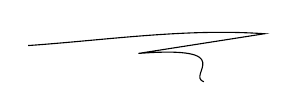
\begin{tikzpicture}[x=1cm,y=1cm]\draw (0,0)..controls(1,.07) and (2,.22)..(3,.15)--(1.4,-.10)..controls(2.7,.0) and (2,-.38)..(2.23,-.46);\end{tikzpicture}}

% @ lower half, heading | text | Graphes cubiques à arête marquée
\uline{\unsure{Graphe cubique|Graphes cubiques|Complexes cubiques} à arête marquée} (ou à triangle marqué avec sommet distingué)

% @ lower left, beside text | diagram | u, v, w ; heavy dot at u
\diagram{\begin{tikzcd}[ampersand replacement=\&,execute at end picture={
\draw (0,0)node[left]{$u$}--(1.03,.85)node[above]{$v$}--(1.27,.25)node[right]{$w$}--cycle;
\fill (0,0) circle (2.1pt);
}]\vphantom{A}\end{tikzcd}}

% @ lower half, construction | text | La description de cette structure
La description de cette structure se déduit de la description précédente en termes de $\{P_u,P\text{ torseur sous }\Psi_{Q_u}\}$ en se donnant de plus un élément fixé \inserted{$t$} de $Q_u$, de sorte que la donnée de $Q_u$ \inserted{de cardinal 5} revient à celle de $Q_u-\{t\}\deleted{\unsure{\mathrm{de}}}=P_u$ de cardinal 4. Alors
% @ lower third, projection below isomorphism | diagram | Ψ(Qᵤ), F₂ to powers Pᵤ and Qᵤ
\diagram{\begin{tikzcd}[ampersand replacement=\&,row sep=tiny]
\Psi(Q_u)\arrow[r,"\sim"]\arrow[r,phantom,"\deleted{\unsure{\simeq|\leftarrow}}"{above,pos=.22}] \&\mathbb F_2^{P_u}\\
\mathbb F_2^{Q_u}\arrow[u,phantom,"\subset"{description,rotate=-18}]\arrow[ur,"\mathrm{proj}"'] \&
\end{tikzcd}}
% @ lower third, torsor | text | donc la donnée du torseur
, donc la donnée du torseur $P$ sous $\Psi(Q_u)$ équiv. à celle d'un torseur $P$ sous $\mathbb F_2^{P_u}$ -- i.e. \inserted{$(P_u,P)\longleftarrow$} un ens. \inserted{$\widetilde P_u$} de cardinal 8 avec $\sigma$ autom involutif ss pt fixe.

% @ foot, augmentation | text | Considérons ε
\deleted{Alors} \deleted{\unsure{SPS}} Considérons $\varepsilon:\mathbb F_2^{P_u}\longrightarrow\mathbb F_2$, alors on a
% @ foot, decomposition | display | C as disjoint union
\[
C\simeq\{u\}\amalg\overbrace{\bigl(P\times_{\mathbb F_2^{P_u}}(\mathbb F_2,\varepsilon)\bigr)}^{\{v,w\}}
\amalg\deleted{\unsure{P}}\overbrace{\left(\coprod_{i\in P_u}\bigl(P\times_{\mathbb F_2^{P_u}}(\mathbb F_{2},p_i)\bigr)\right)}^{\widetilde P_u}
\amalg\overbrace{P}^{E}
\]
% archive sheet number: 23
\scanpage{25}\mspage{19}
% @ top, a | text | u,v,w liés
a) $u,v,w$ liés deux à deux

% @ top, b | text | u lié aux éléments
b) $u$ lié aux éléments de $\widetilde P_u$, $v$ et $w$ non liés à ces éléments.

% @ top, c | text | u non lié aux él.
c) $u$ non lié aux él. de \deleted{\unsure{$E$}} $P$. Si $v\in P\wedge_{\mathbb F_2^{P_u}}(\mathbb F_2,\varepsilon)$, il est lié à $x\in P$ sss il est dans l'image de $x$ par $P\longrightarrow P\wedge_{\mathbb F_2^{P_u}}(\mathbb F_2,\varepsilon)$.

% @ upper third, d | text | Deux éléments
d) Deux éléments de $\widetilde P_u$ liés sss ils sont conjugués par $\sigma$, i.e. \deleted{\unsure{qu'ils}} \deleted{\unsure{liés par un}} sont $\in$ des $=$ \unsure{sommands|sommants} $P\wedge_{\mathbb F_2^{P_u}}(\mathbb F_2,p_i)$ $(i\in P_u)$ et sont distincts (i.e. sont distincts et ont $=$ image dans $\widetilde P_u\text{---}P_u$)

% @ upper middle, e | text | Un él. a
e) \deleted{Deux} Un él. $a$ de $\widetilde P_u$ lié à un él. $x$ de $P$ sss, si $a\in P\wedge_{\mathbb F_2^{P_u}}(\mathbb F_2,p_i)$, $a$ est dans l'image de $x$.

% @ upper middle, f | text | x et y
f) $x$ et $y\in P$ sont liés sss, posant $x-y=u$, \deleted{\unsure{$x$}}\inserted{$u$} est de la forme \deleted{\unsure{$e_1,e_2,e$|$e'_1,e_2,\ldots$} $e'_i$ $(i\in P_u)$,}
% @ above the fold, two sums | display | e′ᵢ ; e′₀
\[
e'_i=\sum_{j\in P_u-\{i\}}e_{\unsure{i|j}}\quad\text{\uline{ou}}\quad\deleted{\Sigma}\ e'_0=\sum_{i\in I}e_i
\]

% @ lower half, ruled corollary | text | Corollaire Le groupe des autom.
% @ left of corollary, first vertical | drawing | vertical line beside first paragraph
\noindent\makebox[0pt][r]{\raisebox{-4\baselineskip}[0pt][0pt]{\tikz\draw (0,0)--(0,2.1);}\hspace{.6em}}\uline{Corollaire} Le groupe des autom. \inserted{$W_{\{v,w\}=\alpha}$} de $(C,\{v,w\})$ (où $\{v,w\}$ est une arête marquée) est isom. au groupe des couples $(\rho,\varphi)$, où $\rho$ \inserted{$\in\unsure{\mathfrak S|\mathscr S}_{P_u}$} est un autom. de \deleted{groupe} $P_u$, et $\varphi$ un $\bar\rho$-autom de $P$. Donc on a une suite exacte \inserted{(splittée)}
% @ lower third, exact sequence | diagram | 1, F₂, Wα, S, 1
\diagram{\begin{tikzcd}[ampersand replacement=\&,column sep=large]
1\arrow[r,dash]\&(\mathbb F_2^{P_u})^{\deleted{\unsure{P|F}}}\arrow[r]\&W_\alpha\arrow[r,dash]\&\mathfrak S_{P_u}\arrow[r,dash]\&1
\end{tikzcd}}
% @ lower third, identification | text | et Wα est isom.
% @ left of identification | drawing | second vertical line
\noindent\makebox[0pt][r]{\raisebox{-1.3\baselineskip}[0pt][0pt]{\tikz\draw (0,0)--(0,1.1);}\hspace{.6em}}et $W_\alpha$ est isom. au groupe de Weyl $W_{B_4}$ de $B_4$ $(\simeq\mathrm{so}(9))$

% @ foot, root count and change of situation | text | Ce système de racines
Ce système de racines $B_4$ a 32 racines \inserted{(mais pas ttes de $=$ \unsure{longr.|longueur} !)} qu'on aimerait retrouver plongé dans $E_6$. Il vaut mieux, pour éliminer les longueurs inégales, épingler légèrement la situation,
% archive sheet number: 24
\scanpage{26}\mspage{20}
% @ top, continuation | text | en épinglant le triangle
en épinglant le triangle $u,v,w$ i.e. l'arête $(v,w)$ par choix d'une ``origine'' $v$ -- i.e. partant d'un \uline{arc} \inserted{$\vec\alpha$} plutôt que d'une arête $\alpha$. \deleted{Alors}, Cel\unsure{a} signifie aussi (comme $\{v,w\}=P\wedge_{\mathbb F_2^{P_u}}(\mathbb F_2,\varepsilon)$) qu'on a restreint le groupe structural de $\mathbb F_2^{P_u}$ : $\Psi_{P_u}=\operatorname{Ker}(\mathbb F_2^{P_u}\overset{\varepsilon}{\longrightarrow}\mathbb F_2)$. On trouve donc l'extension splittée
% @ top third, extension | diagram | 1, Ψ, W, symmetric group, 1
\diagram{\begin{tikzcd}[ampersand replacement=\&,column sep=large]
1\arrow[r,dash]\&\Psi_{P_u}\arrow[r,dash]\&W_{\vec\alpha}\inserted{=W_t}\arrow[r,dash]\&\unsure{\mathfrak S|\mathscr S}_{P_u}\arrow[r,dash]\&1
\end{tikzcd}}
% @ upper middle, identification | text | donc
donc
% @ upper middle, W | display | W of the directed edge
\[
W_{\vec\alpha}\simeq W_{D_4}
\]
\margin{autom de $C$ qui sont l'identité sur $t=\{u,v,w\}$}

% @ middle, root count | text | groupe de Weyl de D₄
groupe de Weyl de $D_4$ $(\simeq\mathrm{so}(8))$. Ce syst. de racines (ttes de $=$ longueur) à $\frac{8.7}{2}-4=24$ racines. On retrouve $W_t$ par une description plus symétrique (en $u,v,w$) plus bas, ainsi qu'une description plausible du syst de 24 racines de type $D_4$ associé à un triangle \ldots.

% @ right margin, drawings and words | text | Complexe cubique avec balai
\margin{Complexe cubique avec balise \unsure{marquée|marqué} ou à \inserted{couple de} triangles incidents marqué}
% @ right, beside first phrase | diagram | v w above u ; lower end a
\diagram{\begin{tikzcd}[ampersand replacement=\&,execute at end picture={
\draw[thick](0,1)node[above left]{$v$}--(.6,1)node[above right]{$w$}--(.29,.53)node[left]{$u$}--cycle;
\draw[thick](.29,.53)--(.31,-.13)node[below right]{$a$};}]\vphantom{A}\end{tikzcd}}
% @ right, beside second phrase | diagram | v w, u, a b
\diagram{\begin{tikzcd}[ampersand replacement=\&,execute at end picture={
\draw(0,1)node[above left]{$v$}--(.65,1)node[above right]{$w$}--(.31,.49)node[left]{$u$}--cycle;
\draw(.31,.49)--(.04,-.12)node[below left]{$a$}--(.65,-.12)node[below right]{$b$}--cycle;
\fill(.31,.49) circle (1.4pt);}]\vphantom{A}\end{tikzcd}}
% @ centre below paragraph, divider | drawing | two horizontal strokes joined by a loop
\figure{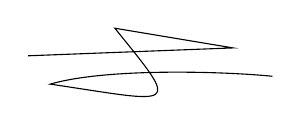
\begin{tikzpicture}\draw(0,0)--(2.6,.1)--(1.1,.35)..controls(1.95,-.7) and (1.9,-.6)..(.28,-.36)..controls(1,-.15) and (2.5,-.2)..(3.1,-.26);\end{tikzpicture}}

% @ lower third, heading | text | Complexe cubique à triangle marqué
\uline{Complexe cubique à triangle \inserted{$t$} marqué}, $t=\{u,v,w\}$.

% @ lower third, opening | text | Équivaut à la donnée
Équivaut à la donnée

% @ foot, a | text | d'un t
a) d'un \deleted{\unsure{ens.}} $t$ de cardinal 3

% @ foot, b | text | d'un vectoriel
b) d'un vectoriel $N$ de dim 2 sur $\mathbb F_2$ ($\Longleftrightarrow$ ens de cardinal 3 savoir $V^*$)

% @ foot, c | text | Un torseur
c) Un torseur $\widetilde P$ sous l'extension canonique
% archive sheet number: 25
\scanpage{27}\mspage{21}
% printed form: music manuscript paper, with blank staves behind the handwriting.
% @ upper staff, continuation of c | text | Ψ tilde de Ψ
$\widetilde\Psi(V,t)$ de $\Psi(V,t)=\operatorname{Ker}\bigl(V^t\overset{\varepsilon}{\longrightarrow}V\bigr)$ par $\mathbb F_2$ \inserted{$(x_i)_{i\in t}\longmapsto\sum x_i$} -- extension à \unsure{splittings|splittages|splitting} \inserted{précisés} sur les $N_i=\operatorname{Ker}\ \Psi(V,t)\overset{p_i}{\longrightarrow}V$ $(i\in t)$ i.e. on a des sous-groupes $N'_i\subset\widetilde\Psi(V,t)$, $N'_i\longrightarrow N_i$. Rappelons que $\widetilde\Psi(V,t)=\bigwedge_{i\in t}p_i^*(\widetilde V)$, où $\widetilde V$ est l'ext. de $V$ par $\mathbb F_2$ qui ne splitte sur aucun sous-groupe $\ne0$ de $V$. On a, alors \unsure{pr tt|notant|pour} $i\in t$

% @ upper middle, eight and four element sets | display | P̃ᵢ, Pᵢ
\[
\begin{aligned}
\overset{\text{``8''}}{\widetilde P_i}&=\widetilde P/N'_i\qquad i\in t\\
P_i&=\widetilde P/\widetilde N_i
\end{aligned}
\]
\margin{$E(i)^*$ ``}\margin{\deleted{\unsure{$E(i)$}}}
% @ right of quotients | text | où Ñᵢ
(où $\widetilde N_i=$ image inverse de $N_i$ dans $\widetilde\Psi$) $=N'_i.\{1,\sigma\}$, \unsure{$\sigma$} -- élém. \unsure{val.} \inserted{$\ne1$ du noyau de $\widetilde\Psi\longrightarrow\Psi$})
% @ centre, set of vertices | display | C ≃ t ⨿
\[
C\simeq t\amalg\left(\coprod_{i\in t}\widetilde P_i\right)
\]

% @ centre, heading | text | La loi du graphe
La loi du graphe est définie ainsi

% @ centre, a | text | les i ∈ t
a) les $i\in t$ sont deux à deux liés

% @ centre, b | text | i est lié
b) $i$ est lié aux él. de $\widetilde P_i$, et non à ceux de $\widetilde P_j$ si $j\ne i$

% @ lower middle, c | text | Si x, y
c) Si \deleted{$x\in\widetilde P_i$,} $\tilde x,\tilde y\in\widetilde P_i$, $x$ et $y$ sont liés sss $y=\sigma x$

% @ lower middle, d | text | Si x̃ ∈ P̃ᵢ
d) Si $\tilde x\in\widetilde P_i,\tilde y\in\widetilde P_j$, $i\ne j$, alors $x$ et $y$ sont liés sss $\exists\,\tilde{\unsure{\vartheta|\theta|\gamma}}\in\widetilde P$ tel que \deleted{$p_i(\tilde\vartheta)=x$,} $p_i(\tilde\vartheta)=\tilde x$, $p_j(\tilde\vartheta)=\tilde y$.

% @ left margin, first slanted note | text | NB P̃ ≃ ens des triangles
\margin{\uline{NB} $\widetilde P\simeq$ ens des triangles $t'$ disjoints de $t$}% slanted
% @ left margin, second slanted note | text | donc Coro Se donner
\margin{donc \uline{Coro} Se donner $(C,t,t')$ avec \unsure{$(t,t')$} triangles disjoints, équivaut à se donner $(t,V)$ ($t$ ens de card 3, $V$ vectoriel de dim 2 sur $\mathbb F_2$)}% slanted

% @ foot, corollary | text | Le groupe des autom
\uline{Coro} Le groupe des autom de $(C,t)$ \deleted{est} est isom au groupe des \deleted{couples} \inserted{triplets} $(\tau,\rho,\varphi)$ d'un autom $\rho$ de $\unsure{\tau|t}$ de $t$, d'un autom $\rho$ de $V$, et d'un \deleted{\unsure{$(\tau,\rho)$}} $\lambda_{\tau,\rho}$-autom de $\unsure{\widehat P|\widetilde P}$, où $\lambda_{\tau,\rho}$ est l'autom de \deleted{\unsure{$V_t$|$\Psi$}} $\Psi(V,t)$ induit par \deleted{$(\rho,\tau)$} $(\tau,\rho)$. Donc
% @ bottom staff, exact sequence | diagram | 1, P̃, W, S_t × S_V*, 1
\diagram{\begin{tikzcd}[ampersand replacement=\&,column sep=small]
1\arrow[r]\&\widetilde{\unsure{P|\Gamma}}\arrow[r]\&W_t\arrow[r]\&\overset{\simeq\mathfrak S_3\times\mathfrak S_3}{\unsure{\mathfrak S|\mathscr S}_t\times\mathfrak S_{V^*}}\arrow[r,dash]\&1
\end{tikzcd}}
% archive sheet number: 26
\scanpage{28}\mspage{22}
% printed form: blank music staves.
% @ top, continuation | text | (extension splittée). Sauf erreur
(extension splittée). Sauf erreur, ce groupe est le groupe de Weyl complété (par autom. ext.) de $D_4$ (le gpe des autom. ext. de $D_4$ correspondant à $\unsure{\mathfrak S|\mathscr S}_t$).

% @ upper third, dark interline | text | Donc cat. des syst.
Donc cat. des syst. de racines de type $D_4\simeq$ cat. des complexes cubiques munis d'un triangle

% @ upper third through centre | text | Précisons comment on peut associer
Précisons comment on peut associer un syst. de 24 racines (de type $D_4$) à un triangle $t$ dans $C$. Rappelons qu'à la situation $(C,t=\{u,v,w\})$ on associe \deleted{\unsure{des bij pour} $i,j\in t$, $i\ne j$, \unsure{entre}} \inserted{un syst. transitif d'isom} \deleted{\unsure{entre}} les ens $B(i)$ $(i\in t)$, où $B(i)\subset\unsure{\mathfrak P|\mathcal P}_2(\widetilde P_i)$ est formé des \deleted{couples} paires $(\tilde x,\tilde y)$ d'éléments non liés ; $\{x,y\}\in B(i)$ et $\{x',y'\}\in B(j)$ $(i\ne j)$ sont associés sss \deleted{\unsure{tt} $x\in$} $x,y$ \uline{sont liés} à $x',y'$
% @ middle, common set | text | Si on désigne par B
\deleted{\unsure{Soit B|Si $B$}} Si on désigne par $B$ l'ens \deleted{des} ``commun'' des $B(i)$, i.e. l'ens des parties \inserted{$b$} à 6 élts de $C$ mutuellement non liés (i.e. des bases) telles que $b\cap\underset{\substack{\simeq\\\widetilde P_i}}{\widehat E(i)^*}$ soit de cardinal 2 pour tt $i\in t$, on voit que \inserted{$\forall i\in t$} $B\overset{\sim}{\longrightarrow}B(i)$ par $b\longmapsto b\cap E(i)$, et $\operatorname{Card}B=\operatorname{Card}B(i)=\frac{8.6}{2}=24$.

% @ lower third, condition | text | La condition écrite sur b
\inserted{Je dis que} La condition écrite sur $b$ \deleted{\unsure{est équiv.}} équivaut à celle que $b\cap E(i)$ soit de cardinal 2 $\forall i\in t$, \deleted{car [il \deleted{faut vérifier} \inserted{suffit} que cette dernière implique que $b\cap t=\varnothing$ \unsure{ou on a} au plus \inserted{$\operatorname{card}$} $(b\cap t)=1$, puisque les pts de $t$ sont mut$^{\mathrm t}$ liés,} \inserted{car} si on avait $u\in t\cap b$, on aurait $\operatorname{Card} E(u)\cap b=\varnothing$] $b$ orthogonale à tout $i\in t$ (on dit que $b$ orthogonale à $t$).
% @ lower left, diagonal NB | text | Comme la somme
\margin{\uline{NB} Comme la somme $\sum_{i\in t}i=\unsure{\eta|\lambda}$ est orth. à \uline{tte} racine, les racines orth. à $t$ sont aussi celles orth. à \uline{deux} él. $i\ne j$ de $t$.}% slanted
% archive sheet number: 27
\scanpage{29}\mspage{23}
% @ top, deferred verification | text | Donc il faudrait vérifier
Donc il faudrait vérifier que l'ens des 24 racines orthogonales à un triangle donné $t$ forment un syst. de racines de type $D_4$ \ldots.

% @ upper right, small block | text | choisissant un sommet
\margin{choisissant un sommet $u\in t$, on prend $E(\unsure{t|u})\subset\frac12E(C)$ engendré par les $x-\frac12\theta$ pour $x\in E(u)^*$, et le syst. de racines engendré par les diff. $\alpha-\beta$, où $\alpha,\beta\in E(u)^*$ sont distincts non liés \ldots.}

% @ left, caption above graph | text | Dg = carroussel
\margin{\unsure{Dg.|$D_4$} = ``\unsure{carroussel|caroussel|carrousel}''}% slanted
% @ left, triangle with pendant pairs | diagram | u,v,w ; λᵤ μᵤ λw μw λv μv
\diagram{\begin{tikzcd}[ampersand replacement=\&,execute at end picture={
\draw(0,1.05)node[left]{$u$}--(1.28,1.1)node[right]{$v$}--(.83,1.86)node[above]{$w$}--cycle;
\draw(0,1.05)--(-.18,.1)node[below]{$\lambda_u$};\draw(0,1.05)--(.11,.1)node[below right]{$\mu_u$};
\draw(1.28,1.1)--(1.06,.07)node[below]{$\lambda_v$};\draw(1.28,1.1)--(1.47,.1)node[below right]{$\mu_v$};
\draw(.83,1.86)--(.69,1.32) (.83,1.86)--(.87,1.21);
\draw(.64,1.0)--(.59,.71)node[below]{$\lambda_w$} (.89,1.0)--(.92,.71)node[below right]{$\mu_w$};}]\vphantom{A}\end{tikzcd}}

% @ upper middle, partition | text | Le syst. formé d'un (C,t,b)
Le syst. formé d'un $(C,t,b)$, $t$ triangle du complexe cubique, $b$ base orth. à $t$, équivaut à celle de $C$ muni d'une base $b$, avec \uline{partition} de $b$ en ens de 3 classes de 2 éléments, \deleted{$C_1,C_2,C_3$} \inserted{soit} $(\unsure{\zeta|\xi}_1,\zeta_2)$, $(\zeta_3,\zeta_4)$, $(\zeta_5,\zeta_6)$, le triangle correspondant étant $\zeta_{12},\zeta_{34},\zeta_{56}$. Pour $b$ fixée, il y a $\binom62\binom42\frac1{3!}=15$ telles partitions, donc pour $C$ fixé il y a $\underset{2^3.3^3.5}{\underbrace{72.15}}$ tels couples $(t,b)$, \deleted{\unsure{soit} (comme ils sont} (manifestem$^{\mathrm t}$ tous conjugués), avec un groupe de stabilité qui est une extension de $\unsure{\mathfrak S|\mathscr S}_3$ par $\mathfrak S_2^3$ (en fait, gpe de Weyl de $B_3\simeq\mathrm{so}(7)$).
\margin{(ou encore $\underset{\text{nb de }t}{\underbrace{45}}\times\underset{\substack{\text{nb de }b\text{ pour}\\t\text{ fixé}}}{\underbrace{24}}$)}% slanted

% @ lower third, order and category | text | qui est d'ordre
qui est d'ordre $3!\,2^3=48=2^4.3$ -- on retrouve bien $\operatorname{card}W=(2^3.3^3.5)(2^4.3)=2^7.3^4.5$. La cat. des $(C,t,b)$ équivaut à celle des ens. de cardinal 6 \uline{munis} d'une partition de type $(2,2,2)$, i.e. munis d'un autom inv. d'ordre 2 sans pt fixe. Si on a une \deleted{\unsure{bibase}} $\{b,b'\}$
% archive sheet number: 28
\scanpage{30}\mspage{24 bis}
% printed form: blank music staves.
% @ top, heading | text | Position relative d'un triangle
\uline{Position relative d'un triangle $t$ et d'une base $b$}.

% @ top, root pairing | text | On a
On a $\sum_{i\in t}i=\lambda$ orthogonal aux racines, donc
% @ top, sum | display | Σ i.r_b = 0
\[
\sum_{i\in t}i.r_b=0
\]
% @ upper third, alternatives | text | et comme i r_b
et comme $i\,r_b\in\{0,1,-1\}$ suivant la position relative de $r_b$ et $i$ i.e. \inserted{de} $b$ et $i$, on trouve 2 possibilités (à conjugaison près)

% @ upper third, a | text | i r_b = 0
a) $i\,r_b=0$ $\forall i\in t$, i.e. \deleted{\unsure{de|$E$}} $r_b$ (ou $b$) orthogonal à $t$ : déjà étudié. L'ens de ces $b$ est au nb de 24, stable par passage à l'opposée.
\margin{Ainsi, les bases orthogonales à $t$ sont celles qui sont disjointes de $t$.}% slanted

% @ upper middle, b | text | r_b non orthogonal
b) \deleted{\unsure{\#|$\exists$}} $r_b$ non orthogonal à $t$. Alors on peut écrire $t=\{u,v,w\}$ avec
% @ upper middle, brace at right | display | r_b(u), r_b(v), r_b(w)
\[
\left\{\begin{aligned}
r_b(u)&=1\quad\text{i.e. }u\in b\ \text{i.e. }E(u)\cap b=\varnothing\\
r_b(v)&=-1\quad\text{i.e. }\unsure{u|v}\in b'\ \text{i.e. }\unsure{\widehat E(v)|E(v)}\cap b\ \text{de card. }5\\
r_b(w)&=0\quad\text{i.e. }w\notin b\cup b'\ \text{i.e. }E(w)\cap b\ \text{card }2
\end{aligned}\right.
\]
% @ middle, count and question | text | Pour t fixé
Pour $t$ fixé, le nb de ces $b$ est $72-24=48$, se groupant en 6 groupes de 8 bases $b$, pour lesquels $u,v,w$ sont fixés. Comment paramétrer ces 8 bases ? On note que \inserted{l'intersection de} $E(w)$ avec $b$ et $b'$ est de cart. 2, il contient exactement un pt $u'\in b'$ et un $v'\in b$, et ces deux sont liés. Donc les \unsure{8} choix s'obtiennent en choisissant \deleted{1°) le triangle \unsure{$s$|$S$|6} $(w,u',v')$ parmi les quatre triangles $\ne(w,v,u)$ ayant $w$ comme sommet 2°) un des huit sommets de \inserted{$E(w)^*$} \unsure{5 distincts de $w$ comme étant $u'$|5 distincts de $u$ comme étant $u'$},} la base $b$ est l'unique base \inserted{de $C$} pour laquelle $u\in b$, $u'\in b'$,

% @ foot, reformulation | text | Le choix d'un couple
Le choix d'un couple $(t,b)$ en position non orthogonale équivaut donc à celle d'un triangle épinglé $\{u,v,w\}$ et d'un $u'\in E(w)^*$ (Nb : $27.10.1.8$)
% archive sheet number: 29
\scanpage{31}\mspage{24 ter}
% @ top and middle, subgroup | text | le groupe d'autom.
le groupe d'autom. de $(C,t,b)$ est le sous-groupe de $W_{D_4}$ formé des autom de $(E(w)^*,\sigma,-)$ qui invarient $v'\in E(w)^*$, c'est donc aussi le groupe $W_{D_3}$ des autom de $\bigl(E(w)^*-\{\unsure{w'|v'|u'}+ \sigma v'\},\sigma\bigr)$ qui correspondent à un nb pair de chgts de signes. Quel est le syst. de racines de type $D_3$ associé (formé de 12 racines) ? On trouve \deleted{sans doute le} syst. des racines de la forme $\alpha-\beta$, où $\alpha,\unsure{\beta'|\beta}\in E(w)^*\smallsetminus\{v',\sigma v'\}$ \inserted{sont non liés -- il ne dépend que de l'ens $\{s,t\}$ des}
\margin{deux triangles $s,t$ tels que $s\cap t\ne\varnothing$ $s\ne t$ (donc $\operatorname{Card}s\cap t=1$) ce sont aussi les racines orth. à $\{u,v,w,u',v'\}=s\cup t$ i.e. orth. à la fois $s$ et à $t$}% slanted

% @ middle, base with marked elements | text | La donnée de (t,b)
La donnée de $(t,b)$ équivaut aussi à celle d'une \uline{base} $b$, avec deux éléments fixés $\unsure{\zeta|\xi}_1$ et $\zeta_2$ (le triangle $t$ étant alors $(\underset{u}{\underbrace{\zeta_1}},\underset{v}{\underbrace{\zeta'_2}},\zeta_{12})$) -- le gpe des autom de $(C,t,b)$ est donc aussi $\unsure{\mathfrak S|\mathscr S}_4\simeq W_{A_3}$ -- on est dans le cas d'un ``isom. exceptionnel'' $D_3\simeq A_3$. Le nb de ces syst. $t,b$ est $72.6.5=2160=27.10.8$ --
% archive sheet number: 30
\scanpage{32}\mspage{24}
% @ top, continuation | text | au lieu d'une base
au lieu d'une base, il faut en plus se donner un ens. de cardinal 2. (donc le groupe des autom est multiplié par $\unsure{\mathfrak S|\mathscr S}_2$, le nb d'objets est divisé par 2 \ldots).

% @ upper left, bracketed note | text | Étudier position relative
\margin{Étudier position relative d'une racine et d'un triangle}% slanted
% @ upper middle, divider | drawing | short slightly curved horizontal stroke
\figure{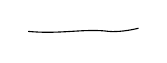
\begin{tikzpicture}\draw(0,0)..controls(.4,-.04) and (.72,.04)..(1.02,0)..controls(1.13,-.01) and (1.28,.01)..(1.4,.04);\end{tikzpicture}}
% @ upper half, triplets | text | Étudions les triples
Étudions les triples $(t,t',b)$, où $(t,t')$ sont deux triangles disjoints et $b$ une base orthogonale à $t$ \uline{et} $t'$ -- ils correspondent à un ens. $I$ de card 6, avec 2 partitions \inserted{$\Pi,\Pi'$} de types $(2,2,2)$, sans classe commune. On trouve que ceci correspond à une structure hexagonale sur $I$ \inserted{à co-triangle inscrit marqué} -- avec comme partitions celles marquées aux traits \rule{1.3em}{.7pt} \inserted{(pour $t$)} et \tikz\draw[decorate,decoration={zigzag,segment length=2pt,amplitude=.5pt}](0,0)--(.45,0); \inserted{(pour $t'$)}. \deleted{\unsure{Les autres paires}} Si on donne $\{t,t'\}$ au lieu de $(t,t')$, on n'a pas à choisir de cotriangle dans l'hexagone.
% @ middle left, hexagon | diagram | vertices 1–6, alternate sides and diagonals
\diagram{\begin{tikzcd}[ampersand replacement=\&,execute at end picture={
\coordinate (a) at (1.45,1.78);\coordinate (b) at (.57,1.88);\coordinate (c) at (-.04,1.15);
\coordinate (d) at (.43,.30);\coordinate (e) at (1.41,.33);\coordinate (f) at (2.00,1.12);
\draw[line width=2pt](a)--(b) (c)--(d) (e)--(f);
\draw[decorate,decoration={zigzag,segment length=2pt,amplitude=.5pt}](b)--(c) (d)--(e) (f)--(a);
\draw(a)--(c)--(e)--cycle (b)--(d)--(f)--cycle;
\draw[dashed](a)--(d) (b)--(e) (c)--(f);
\node[above right]at(a){$1$};\node[above left]at(b){$2$};\node[left]at(c){$3$};\node[below left]at(d){$4$};\node[below]at(e){$5$};\node[right]at(f){$6$};
}]\vphantom{A}\end{tikzcd}}
\margin{penser (plutôt) à l'hexagone dual -- dont les \uline{cotés} sont les él. de $I$ \ldots}% slanted

% @ lower half, completing triangle | text | On trouve que, si t″
On trouve que, si $t''$ est le triangle qui complète $\{t,t'\}$ en un bitriangle $\{t,t',t''\}$, alors $b$ est aussi orth. à $t''$ -- en fait on a la situation d'une base orthogonale à un bitriangle cf plus bas. Pour $b$ fixé, le syst. des $(t,t',t'')$ correspondants est de cardinal $120=5!$ (60 pour $\{t,t'\}$ $=\frac{5!}{2}=$ nb des structures hexagonales sur $I$ de card. 6) en fait en tout \deleted{$120.72=$} $72.5!=\operatorname{card}W/6$ \inserted{$\downarrow$} tels triples]
\margin{$(6=\operatorname{card}\mathfrak S_{\unsure{6|t}}$}% slanted
% @ foot, second count | text | ou nb
ou nb \inserted{(syst aussi :) }
% @ foot, three factors with captions | display | 45 . 32 . 6
\[
\underbrace{45}_{\text{triangles }t}\,.\,\underbrace{32}_{\text{triangles }t'\text{ disj. de }t}\,.\,
\underbrace{6}_{\substack{\text{nb de racines (ou bases)}\\\text{orth. à }t,t'}}
\]
% archive sheet number: 31
\scanpage{33}\mspage{25}
% @ title, first part | text | Complexe cubique à balise marquée
\uline{Graphe cubique à balise marquée}
% @ title, first sign | diagram | triangle and stem, D₄
\diagram{\begin{tikzcd}[ampersand replacement=\&,execute at end picture={\draw(0,1)--(.66,1)--(.32,.54)--cycle (.32,.54)--(.32,-.07);\node[right] at(.9,1){$D_4$};}]\vphantom{A}\end{tikzcd}}
% @ title, second part | text | ou à paire de triangles
\uline{ou à paire} \deleted{\unsure{bitriangle épinglé}} \inserted{de triangles incidents}
% @ title, second sign | diagram | two triangles meeting at a vertex
\diagram{\begin{tikzcd}[ampersand replacement=\&,execute at end picture={\draw(0,1)--(.60,1)--(.30,.57)--cycle (.30,.57)--(.08,.17)--(.55,.17)--cycle;}]\vphantom{A}\end{tikzcd}}
marquée

% @ upper third, first case | text | Cas
Cas
% @ beside Cas | diagram | v,w ; u ; pendant segment
\diagram{\begin{tikzcd}[ampersand replacement=\&,execute at end picture={\draw[thick](0,1)node[above left]{$v$}--(.66,1)node[above right]{$w$}--(.36,.5)node[left]{$u$}--cycle; \draw(.36,.5)--(.36,-.10); \node[above]at(.33,1){$\unsure{\alpha|a}$};}]\vphantom{A}\end{tikzcd}}
, on a une arête marquée $\{v,w\}$, i.e. triangle $\{\deleted{\unsure{t}}u,v,w\}$ à sommet marqué, correspondant à un torseur sous \inserted{un} $\mathbb F_2^{P_u}$. Il faut en plus se donner un él. de $\widetilde P_u$, i.e. un élément de $P_u$ et une trivialisation du $\mathbb F_2$-torseur au dessus -- il reste donc un ens à 3 élmts $R_u=P_u-$

% @ mid-left, linked triangles | diagram | v,w,u,x,y ; dotted sides to y
\diagram{\begin{tikzcd}[ampersand replacement=\&,execute at end picture={
\draw(0,1.55)node[above left]{$v$}--(.79,1.52)node[above right]{$w$}--(.34,.81)node[left]{$u$}--cycle;
\draw(.34,.81)--(.35,-.13)node[below left]{$x$};\draw[dotted](.35,-.13)--(1.02,-.13)node[below right]{$y$}--(.34,.81);
}]\vphantom{A}\end{tikzcd}}
% @ middle to lower half | text | l'ens des 3 triangles
(l'ens des 3 triangles de sommet $u$ distincts de $\{u,v,w\}=t$ et $\{u,xy\}=s$) et un rev. d'ordre 2 de ce dernier, i.e. un torseur sous $\mathbb F_2^{R_u}$. La catégorie des triples $(C,\text{balise})$ est donc \unsure{décrite|discrète}, les autom d'un objet sont un groupe isom. à $\widehat W_{D_3}$ groupe de Weyl élargi (= tous les autom) d'un syst. de racines de type $D_3$,
\margin{balise épinglée donne un groupe d'autom de $(C,\text{bal. ép.})$ qui est $W_{D_3}$ (et non plus $\widehat W_{D_3}$)}% slanted
\inserted{il est de cardinal $3!\,2^3=\uline{48}$} (L'ens $\{v,w\}$ se récupère comme le produit \inserted{de Baer} des 3 \inserted{$\mathbb F_2$-}torseurs indexés par $R_u$ \ldots).

% @ lower third, roots | text | Les racines en question
Les racines en question sont les $\alpha-\beta$, où $\alpha,\beta\in E(\unsure{w|u})^*-\{x,y\}$ sont distincts et non liés.

% @ foot, count | text | Le nb des balises
Le nb des balises de $C$ est
% @ foot, product and labels | display | 45 . 3 . 8 = card W / 48
\[
\underbrace{45}_{\text{triangles }t}.\underbrace{3}_{\substack{\text{sommet }u\\\text{de }t}}.\underbrace{8}_{\in E(u)^*},\quad=\operatorname{card}W_{E_6}:48\qquad\text{OK.}/\ \deleted{\text{\unsure{Le nb des balises}}}
\]
% archive sheet number: 32
